\subsection{Problem}

\renewcommand{\theequation}{\theenumi}
\begin{enumerate}[label=\thesection.\arabic*.,ref=\thesection.\theenumi]
\numberwithin{equation}{enumi}
	\item If the vertices of a parallelogram taken in order are
	\begin{multline}
\vec{A}=\myvec{1\\2} , \vec{B}=\myvec{4\\y} ,\vec{C}=\myvec{x\\6}\text{ and }\vec{D}=\myvec{3\\5}\\\text{find x and y.}
\end{multline}
	The following python code computes the value of x and y used in Fig.\ref{fig:qten}.
	\begin{lstlisting}
	./codes/lines/q10.py
	\end{lstlisting}
	
	\solution In a parallelogram, the diagonals bisect each other. Hence
	\begin{align}
		\vec{\frac{A+C}{2} = \frac{B+D}{2}}
		\\
\therefore \vec{\frac{1+x}{2} = \frac{7}{2}}\text{ and }\vec{\frac{8}{2} = \frac{y+5}{2}} \\
\implies x=6,y=3
\end{align}
	\begin{figure}[!ht]
	\centering
	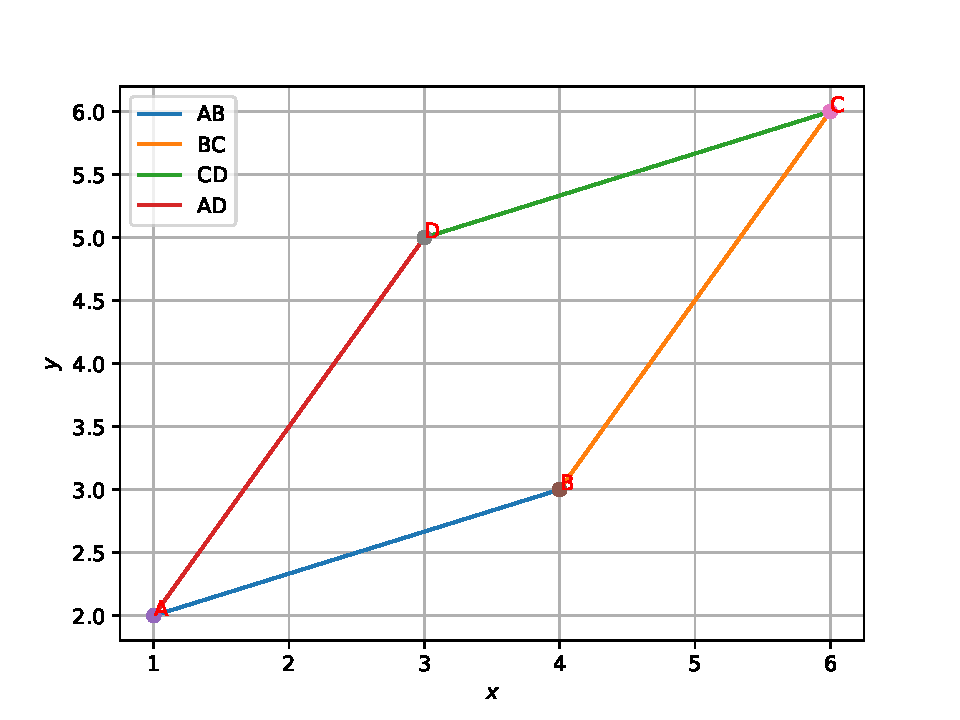
\includegraphics[width=\columnwidth]{./figs/lines/q10.pdf}
	\caption{Parallelogram of Q.3.6.5}
	\label{fig:qten}	
	\end{figure}
	
		
\end{enumerate}
